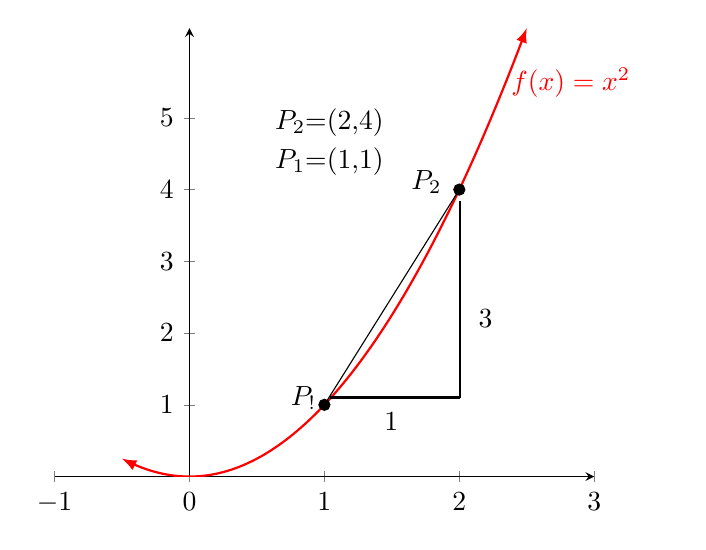
\begin{tikzpicture}
%\draw[step=.5, gray!40, very thin] (0,0) grid (7,5.5);

\begin{axis}[
    domain=-0.5:2.5, samples=100,
    xmin=-1, xmax=3,
    axis x line=bottom,
    axis y line=middle,
    ytick={0,1,2,3,4,5},
]

\addplot [thick, red, latex-latex] {\x^2};
\addplot [black, mark=*] coordinates {(1,1) (2,4)}
node [left, xshift=-0.1cm, yshift=0.1cm] {$P_2$};
\node[text width=.4cm] at (3.2cm,1cm) {$P_!$};


\end{axis}
\draw[line width=1pt]  (5.15,3.5)--(5.15,1) node [right, xshift=0.1cm, yshift=1cm] {$3$};
\draw[line width=1pt]  (5.15,1)--(3.5,1) node [left, xshift=1cm, yshift=-.3cm] {$1$};
\node[text width=.4cm] at (3cm,4.5cm){$P_2$=(2,4)};
\node[text width=.4cm] at (3cm,4cm)  {$P_1$=(1,1)};
\node[text width=2cm,red] at (6.8cm,5cm) {$f(x)=x^2$};
\end{tikzpicture}